\documentclass{article}
\usepackage{geometry}
\usepackage{xcolor}
\usepackage{graphicx}
\usepackage{float,lscape}
\usepackage{listings}
\usepackage{color}
\usepackage{lipsum}% Used for dummy text.
\definecolor{titlepagecolor}{cmyk}{1,.60,0,.40}
\definecolor{namecolor}{cmyk}{1,.50,0,.10}
\definecolor{dkgreen}{rgb}{0,0.6,0}
\definecolor{gray}{rgb}{0.5,0.5,0.5}
\definecolor{mauve}{rgb}{0.58,0,0.82}
\lstset{frame=tb,
  language=Java,
  aboveskip=3mm,
  belowskip=3mm,
  showstringspaces=false,
  columns=flexible,
  basicstyle={\small\ttfamily},
  numbers=none,
  numberstyle=\tiny\color{gray},
  keywordstyle=\color{blue},
  commentstyle=\color{dkgreen},
  stringstyle=\color{mauve},
  breaklines=true,
  breakatwhitespace=true,
  tabsize=3
}
%-----------------------------------------------------------------
\begin{document}
\thispagestyle{plain}
\begin{center}
    \Large
    EFM With Field in 111 Starting With Random and Ground Initial States
    
    \vspace{0.4cm}
    \large
    April 21st, 2016 - May 10th, 2016
    
    \vspace{0.4cm}
    \textbf{Andrew Way}
    
    \vspace{0.9cm}
    \textbf{Overview} \\
    \vspace{5mm}
    The effective field method was used to 2000 iterations to determine the 0 temperature states of 
    the 12x12x12 3D FCC kagome lattice while being subjected to a changing magnetic field along the 111 
    direction. The field was either incremented or decremented in steps of 0.0001. 
    There were 4 cases studied:
    \begin{enumerate}
     \item \textbf{Increasing} magnetic field in the \textbf{111} direction from \textbf{0.00 to 0.05},
     with an initial 
     spin configuration that was a \textbf{ground state} with theta = 0.206275 and phi = 3.11867.
     \item \textbf{Increasing} magnetic field in the \textbf{111} direction from \textbf{0.00 to 0.05},
     with an initial 
     spin configuration that was \textbf{randomly generated}.
     \item \textbf{Decreasing} magnetic field in the \textbf{111} direction from \textbf{0.05 to 0.00},
     with an initial
     spin configuration that was a \textbf{ground state} with theta = 0.206275 and phi = 3.11867.
     \item \textbf{Decreasing} magnetic field in the \textbf{111} direction from \textbf{0.05 to 0.00},
     with an initial
     spin configuration that was \textbf{randomly generated}.
    \end{enumerate}
    Analysis that was performed on the resulting data included the following:
    \begin{itemize}
     \item Plots of magnetization versus field
     \item Plots of energy versus field
     \item Animations of the characteristic 6 spins 
     \item Determination of the number of ``unique'' spins that populate the lattice
     \item Determination of the components of the unique spins
     \item Plots of azimuth and zenith angles of the A, B, C, D, E, and F spins w.r.t. the plane of the 111 normal vector 
    \end{itemize}

\end{center}
\pagebreak
\thispagestyle{plain}
\begin{center}
\LARGE
RUN 1: Increasing Field, Ground State
\end{center}
\paragraph
\large
Steps persist in the energy graphs. This can probably be fixed by increasing precision. 
A sudden drop in energy occurs at field ~0.006. This corresponds to the spin configuration snapping
into a planar state, where the applied field vector intersects the plane. The angle of intersection
is not perpendicular, but looks close to it. Once in the planar state, the spins gradually align
with the field, and nothing else interesting happens. 
\begin{figure}[h]
 \centering 
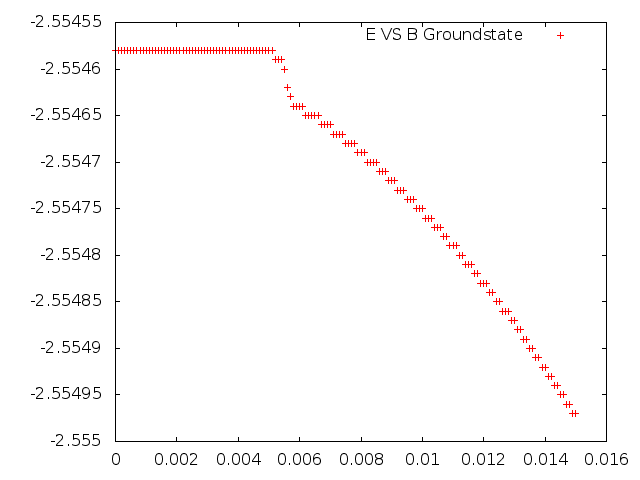
\includegraphics[scale=0.3]{E000to005G.png}
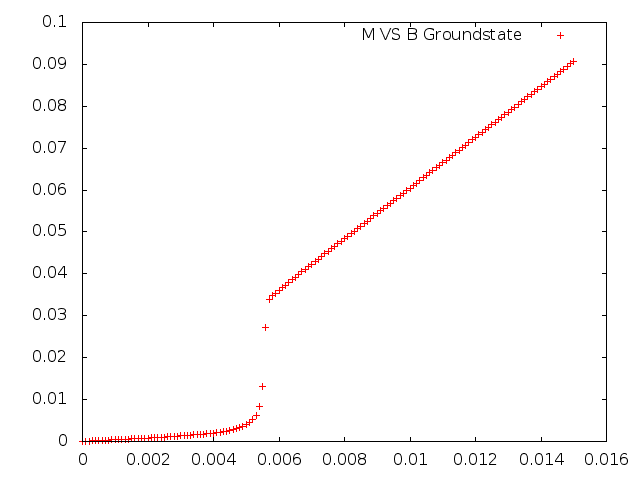
\includegraphics[scale=0.3]{M000to005G.png}
\caption{Energy vs increasing field and Magnetization versus increasing field}
\end{figure}
\begin{figure}[ht]
\centering
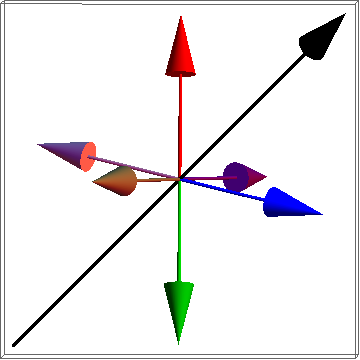
\includegraphics[scale=0.27]{1S000to005G.png}
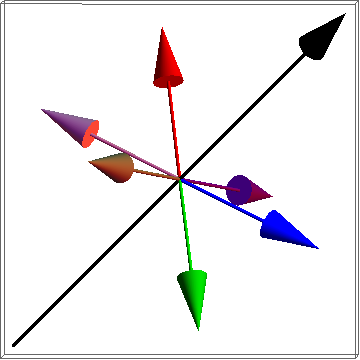
\includegraphics[scale=0.27]{2S000to005G.png}
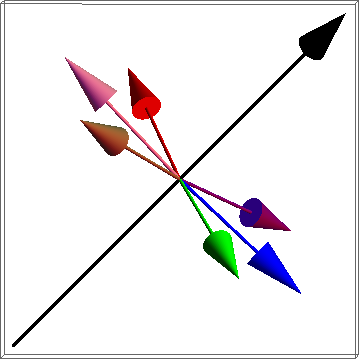
\includegraphics[scale=0.27]{3S000to005G.png}
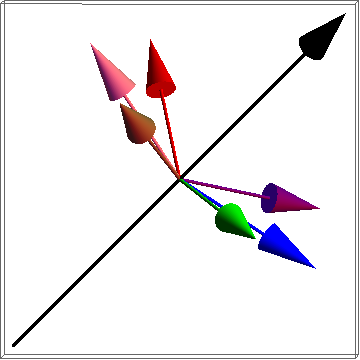
\includegraphics[scale=0.27]{4S000to005G.png}
\caption{Snapshots of the 6 characteristic spins of the lattice at B=0, B=0.0052, B=0.0077, and B=0.05}
\end{figure}
\pagebreak

\begin{figure}
\centering
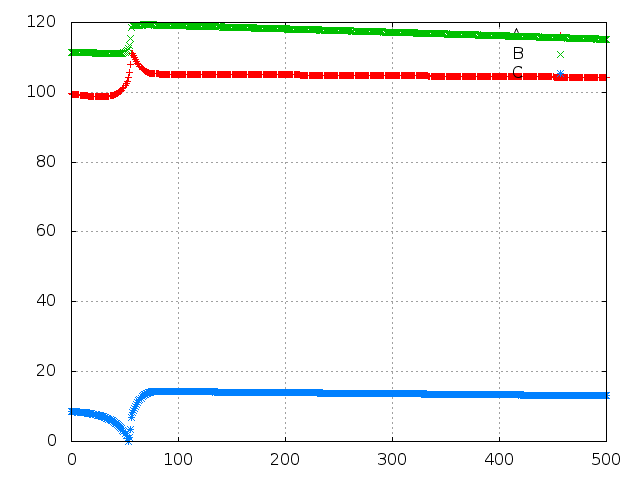
\includegraphics[scale=0.5]{azim000to005.png}
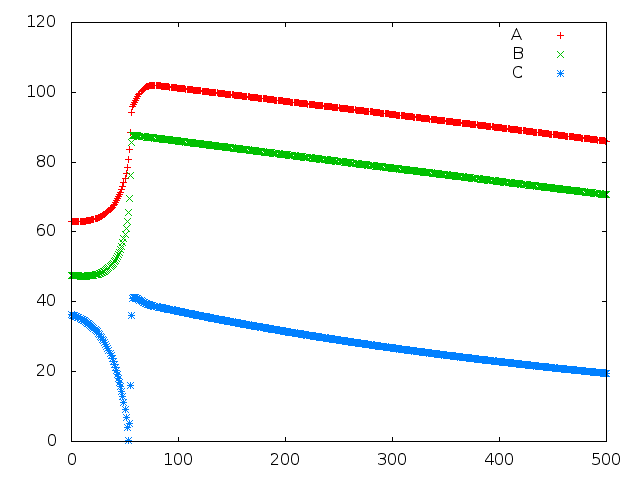
\includegraphics[scale=0.5]{zen000to005.png}
\caption{The angles are those between a chosen vector lying in the plane intersected by 111,
and a projection of each of the A, B, and C spins. Azimuthal angles are followed by zenith angles.}
\end{figure}
\pagebreak

\begin{center}
 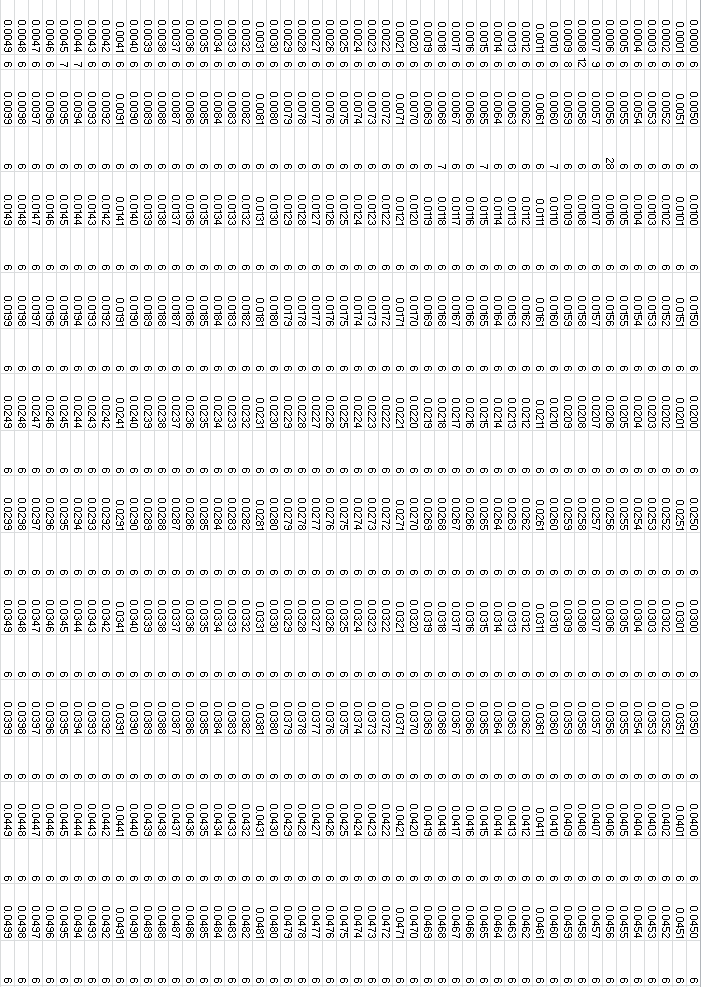
\includegraphics[keepaspectratio,scale=0.58]{000to005SpinChart.png}
\end{center}
\pagebreak
\thispagestyle{plain}
\begin{center}
\LARGE
RUN 2: Decreasing Field, Ground State
\end{center}
\paragraph
\large
Steps persist in the energy graphs. Increasing precision can probably fix this. Unlike the case where the
field was increased, a sudden transition does not occur within the spin configuration when decreasing
the field. The field is initially at its highest, and the spins are partially aligned with the field. 
As the field is lowered, the spins gradually relax to a planar state, and do not return to the 
ground state that is typically observed at near zero or zero field. 
\begin{figure}[h]
 \centering 
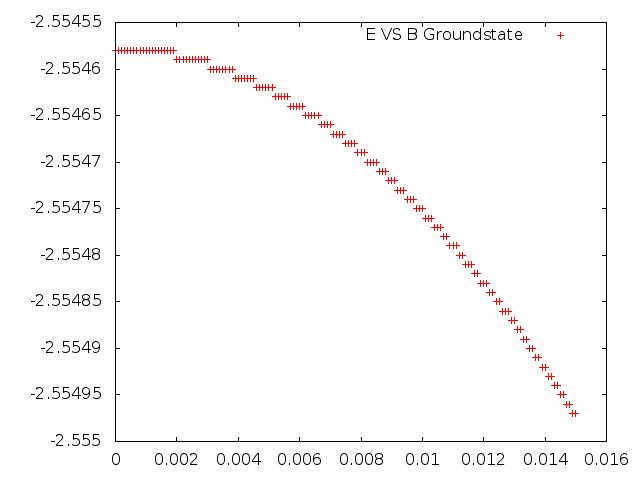
\includegraphics[scale=0.3]{E005to000G.png}
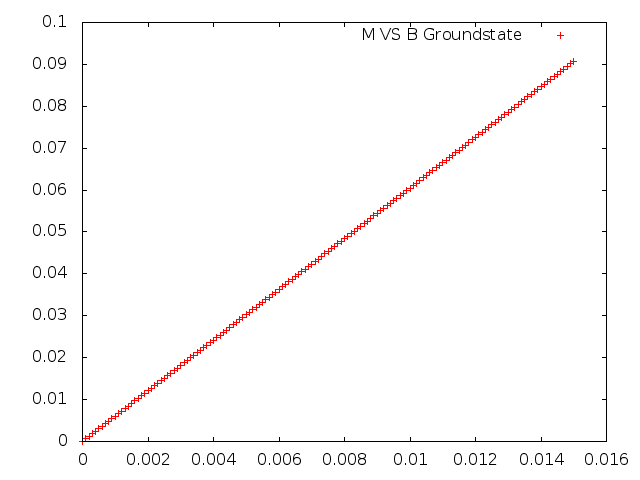
\includegraphics[scale=0.3]{M005to000G.png}
\caption{Energy vs decreasing field and Magnetization versus decreasing field}
\end{figure}
\begin{figure}[ht]
\centering
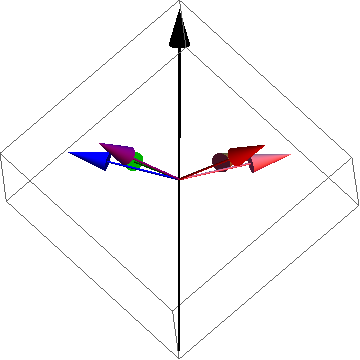
\includegraphics[scale=0.27]{1S005to000G.png}
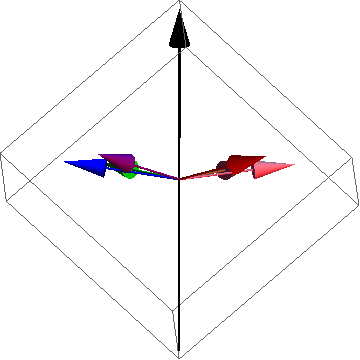
\includegraphics[scale=0.27]{2S005to000G.png}
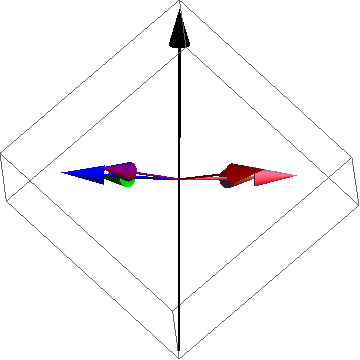
\includegraphics[scale=0.27]{3S005to000G.png}
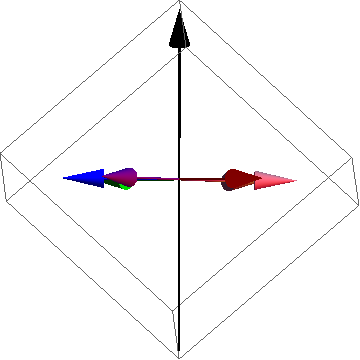
\includegraphics[scale=0.27]{4S005to000G.png}
\caption{Snapshots of the 6 characteristic spins of the lattice at B=0.05, B=0.0309, B=0.01, and B=0.00}
\end{figure}
\pagebreak
\begin{figure}
\centering
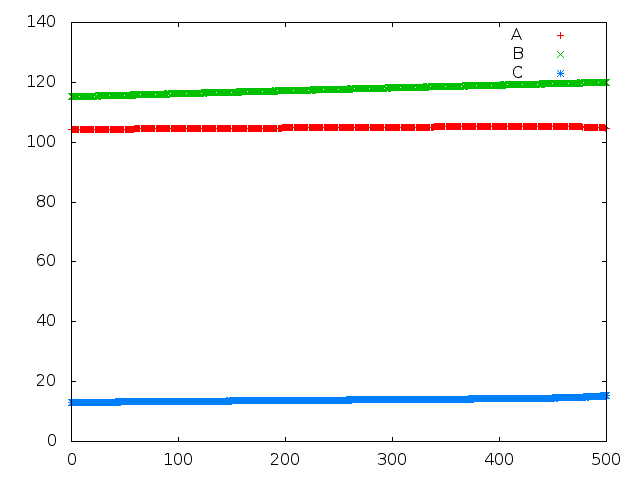
\includegraphics[scale=0.5]{azim005to000.png}
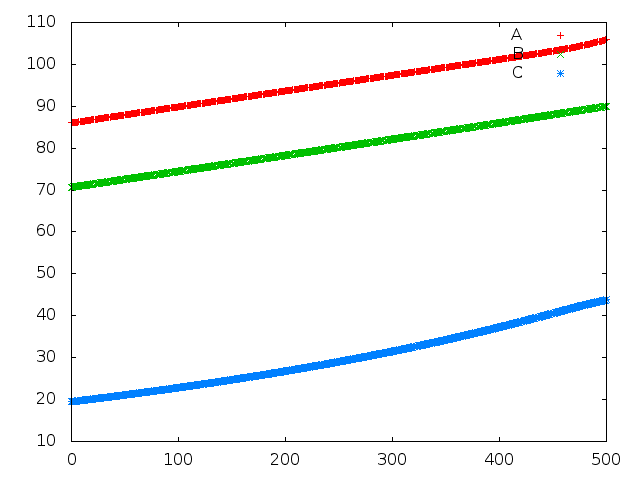
\includegraphics[scale=0.5]{zen005to000.png}
\caption{The angles are those between a chosen vector lying in the plane intersected by 111,
and a projection of each of the A, B, and C spins. Azimuthal angles are followed by zenith angles.}
\end{figure}
\pagebreak
\begin{center}
 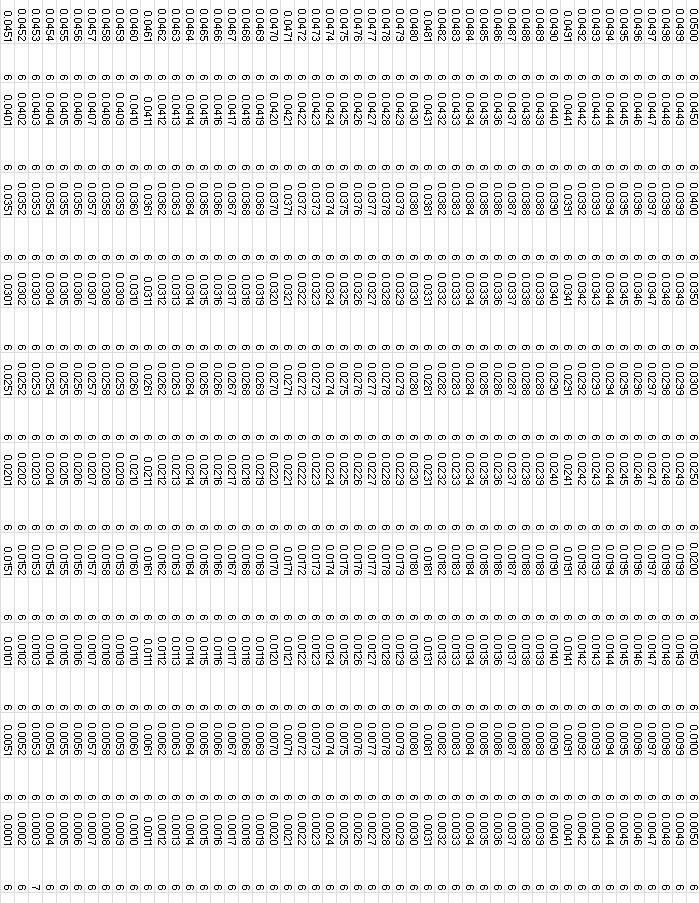
\includegraphics[keepaspectratio,scale=0.83]{005to000SpinChart.png}
\end{center}
\pagebreak

\thispagestyle{plain}
\begin{center}
\LARGE
RUN 3: Increasing Field, Random State
\end{center}
\paragraph
\large
Very similar to run 1, where the lattice starts off at a ground state configuration and snaps into
a planar configuration, followed by gradual alignment with the field. Note: the first data point
in the energy and magnetization plots were removed since it was much higher than any other points
on the graph, which caused the plot to become flattened in order to fit the entire range of data onto
the same plot. This is likely due to the fact that 2000 iterations is insufficient for the energy to
be minimized, and so starting from a random initial configuration causes the energy of the lattice at
the first field value (B=0) to be much higher than the ground state since it has yet to become a 
ground state. 
\begin{figure}[h]
 \centering 
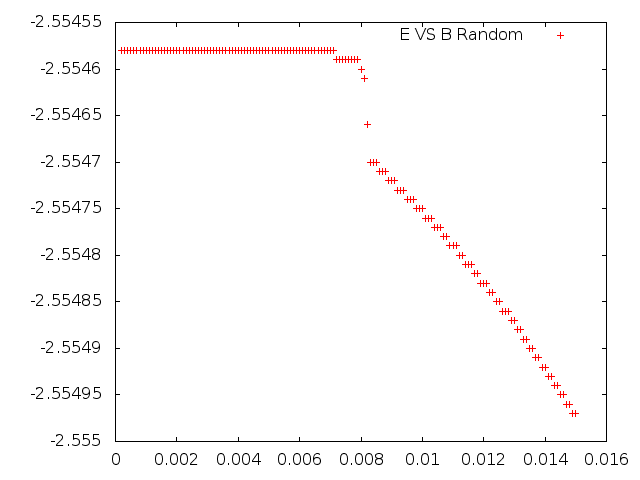
\includegraphics[scale=0.3]{E000to005R.png}
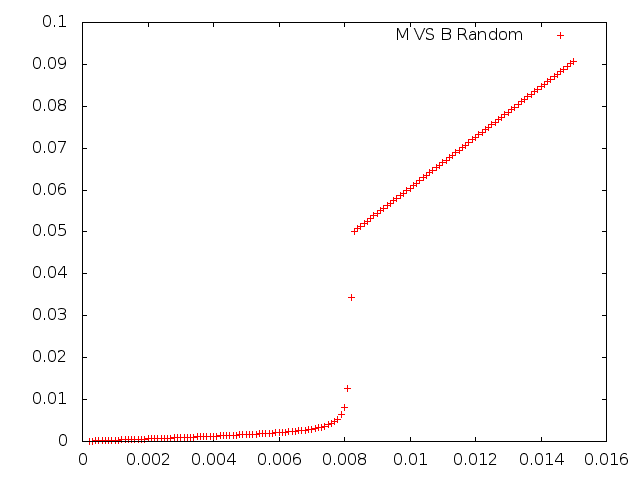
\includegraphics[scale=0.3]{M000to005R.png}
\caption{Energy vs increasing field and Magnetization versus increasing field}
\end{figure}
\begin{figure}[ht]
\centering
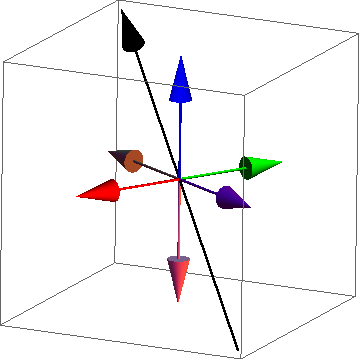
\includegraphics[scale=0.27]{1S000to005R.png}
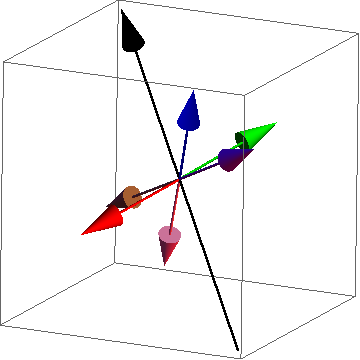
\includegraphics[scale=0.27]{2S000to005R.png}
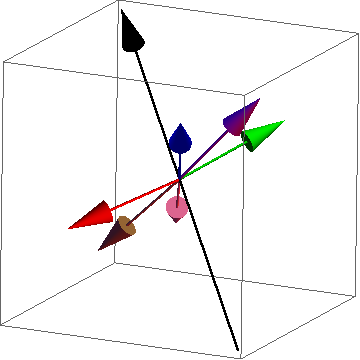
\includegraphics[scale=0.27]{3S000to005R.png}
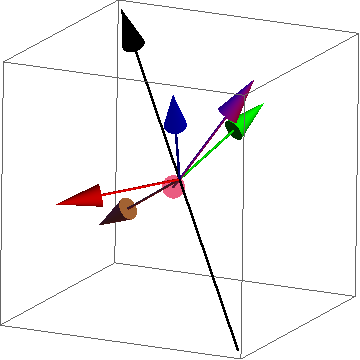
\includegraphics[scale=0.27]{4S000to005R.png}
\caption{Snapshots of the 6 characteristic spins of the lattice}
\end{figure}
\begin{figure}
\centering
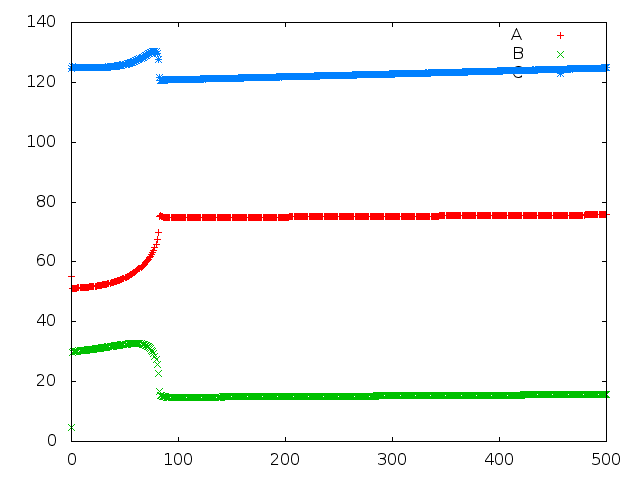
\includegraphics[scale=0.5]{azim000to005R.png}
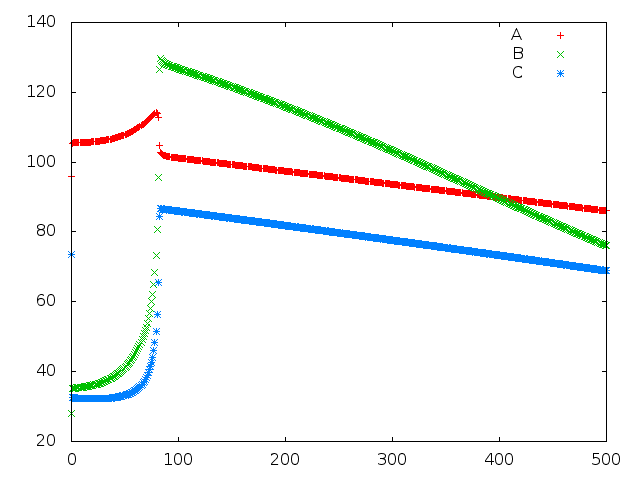
\includegraphics[scale=0.5]{zen000to005R.png}
\caption{The angles are those between a chosen vector lying in the plane intersected by 111,
and a projection of each of the A, B, and C spins. Azimuthal angles are followed by zenith angles.}
\end{figure}
\pagebreak
\pagebreak
\begin{center}
 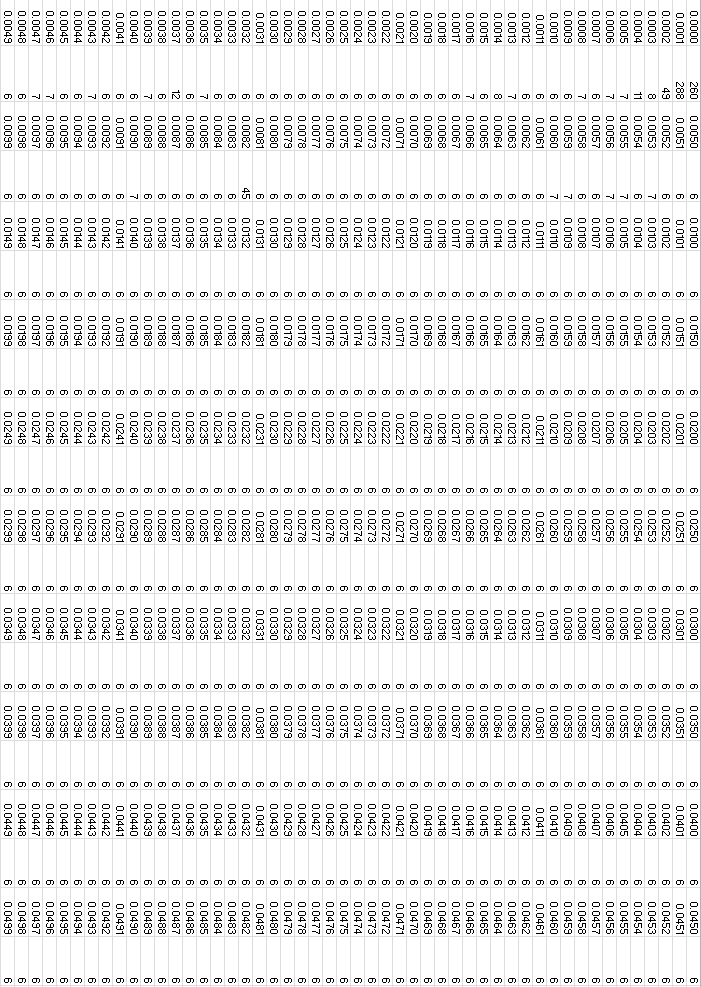
\includegraphics[keepaspectratio,scale=0.58]{000to005RSpinChart.png}
\end{center}


\thispagestyle{plain}
\begin{center}
\LARGE
RUN 4: Decreasing Field, Random State
\end{center}
\paragraph
\large
Between the first two images of the 6 spins, there is little difference even though the field had
changed by about 0.03. At ~0.21, the 6 spins undergo sudden and rapid changes in orientation. Eventually,
the 6 spins rest in a near planar state, and gradually relax to a full planar state at B=0. When 
referring to the spin chart, it's clear that trying to visualize the entire lattice by choosing 6
spins won't work, since there are far more than 6 spins for the majority of fields. 
An alternate approach was used, which involved looking at a small, manageable section of the entire 
lattice. 

\begin{figure}[h]
 \centering 
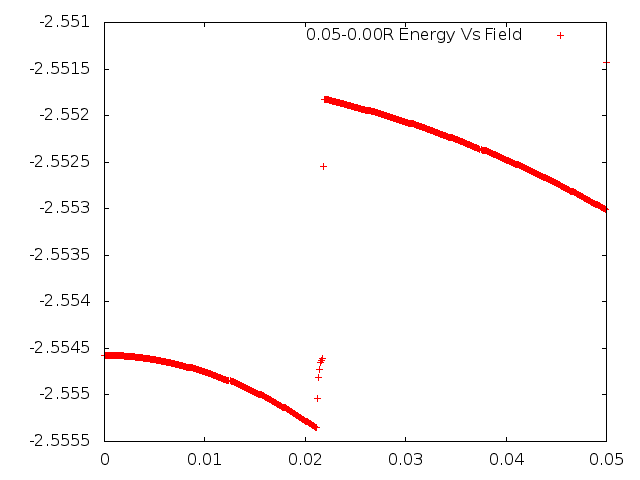
\includegraphics[scale=0.3]{E005to000R.png}
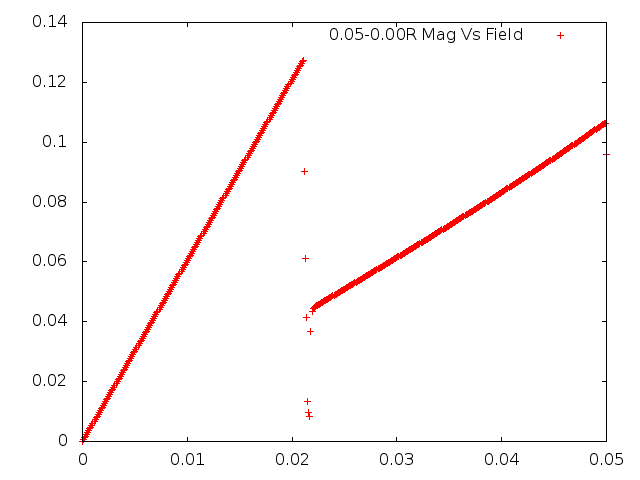
\includegraphics[scale=0.3]{M005to000R.png}
\caption{Energy vs decreasing field and Magnetization versus decreasing field}
\end{figure}
\begin{figure}[ht]
\centering
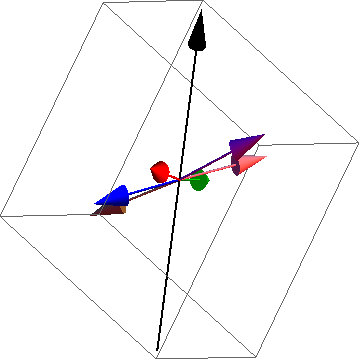
\includegraphics[scale=0.27]{1S005to000R.png}
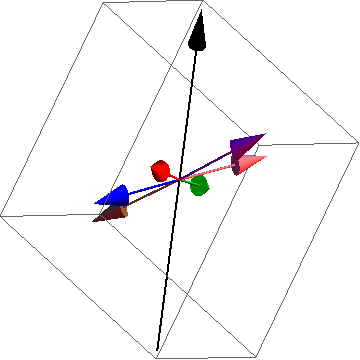
\includegraphics[scale=0.27]{2S005to000R.png}
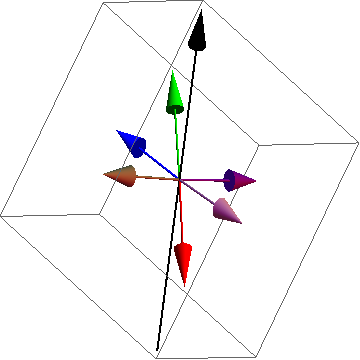
\includegraphics[scale=0.27]{3S005to000R.png}
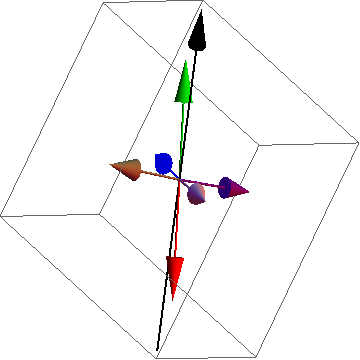
\includegraphics[scale=0.27]{4S005to000R.png}
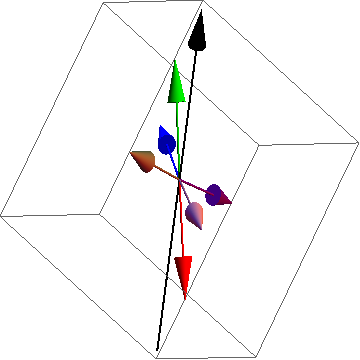
\includegraphics[scale=0.27]{5S005to000R.png}
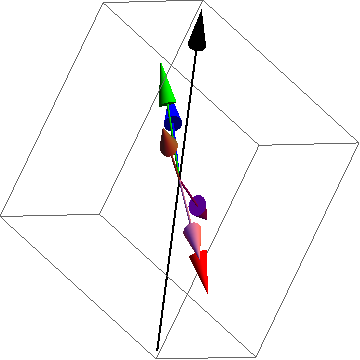
\includegraphics[scale=0.27]{6S005to000R.png}
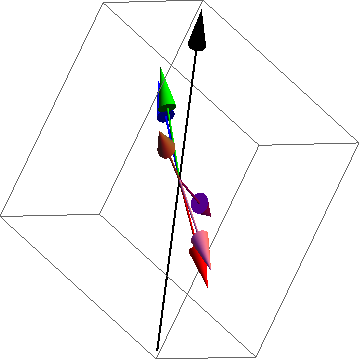
\includegraphics[scale=0.27]{7S005to000R.png}
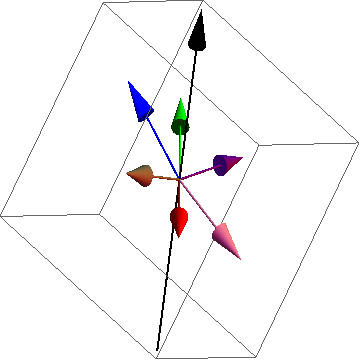
\includegraphics[scale=0.27]{8S005to000R.png}
\caption{Snapshots of the 6 characteristic spins of the lattice over the course of increasing field}
\end{figure}
\pagebreak

\begin{figure}
\centering
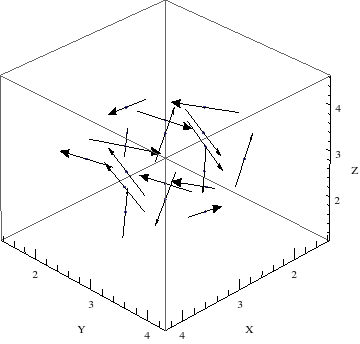
\includegraphics[scale=0.7]{1Sect005to000R.png}
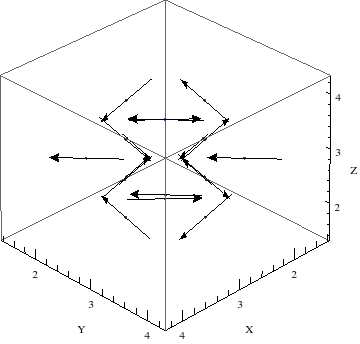
\includegraphics[scale=0.7]{2Sect005to000R.png}
\caption{Visualization of a small section of the entire lattice used in RUN 3. The spins are initially
highly disordered, until they snap into a final planar configuration.}
\end{figure}

\begin{figure}
\centering
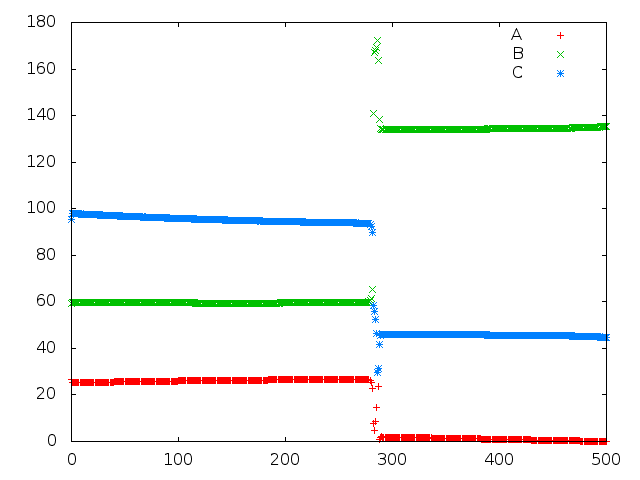
\includegraphics[scale=0.5]{azim005to000R.png}
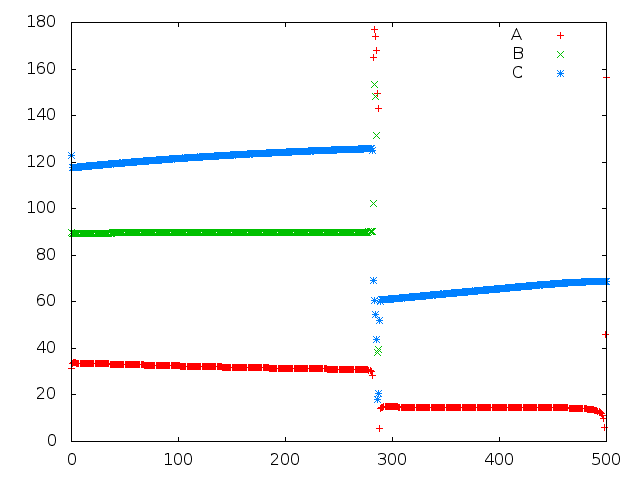
\includegraphics[scale=0.5]{zen005to000R.png}
\caption{The angles are those between a chosen vector lying in the plane intersected by 111,
and a projection of each of the A, B, and C spins. Azimuthal angles are followed by zenith angles.}
\end{figure}
\pagebreak

\pagebreak
\begin{center}
 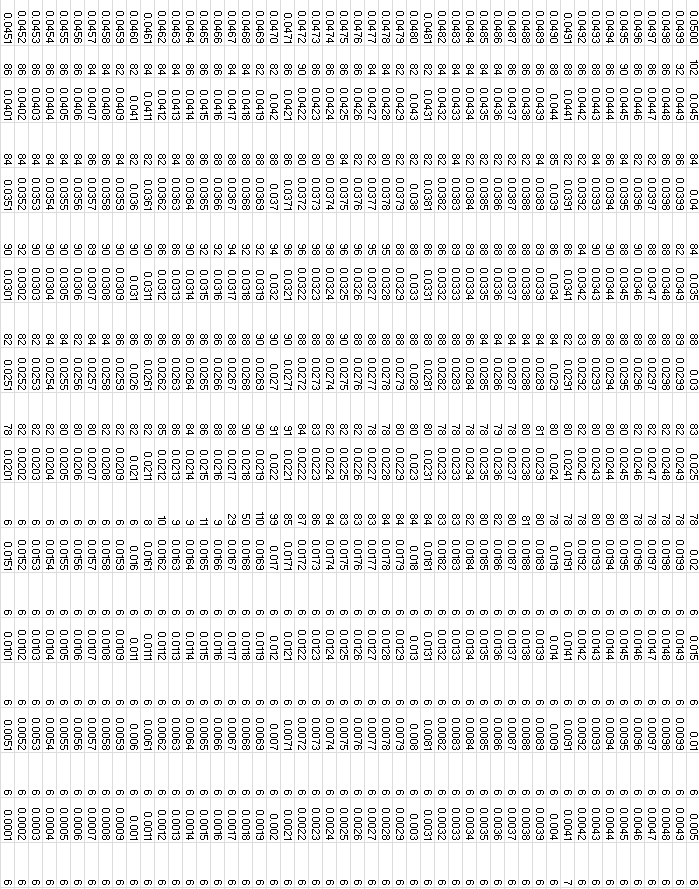
\includegraphics[keepaspectratio,scale=0.85]{005to000RSpinChart.png}
\end{center}
\pagebreak


\begin{center}
\LARGE\textbf{Appendices} \\
\end{center}
\Large
Appendix A - Finding Unique Spins
\large
\paragraph{Overview}
This script finds all confxxxx.f90 files in the current directory, scans through each of them,
and finds each unique spin that occurs within that conf file. The script outputs the name
of the conf file followed by the number of unique spins that exist in that file,
and each unique spin that exists in the file. A spin is considered unique when it has never 
been encountered before; that is, it does not already exist in a temporary file that stores all 
unique spins encountered for the current conf file. A spin is considered unique when it does not
match any of the spins contained within this file up to some pre-determined decimal places. 
If the number of unique spins within the conf file surpasses a number of spins
(specified by the first argument) the spins will not be added to resulting uniqueSpins.txt file. 
\lstset{language=BASH}
\begin{lstlisting}
#!/bin/bash
#findUnique.sh Andrew Way arw405@mun.ca

if [[ $# < 2 ]];then
echo "Usage: ./findUniqueRx.sh uniqueSpinLimit NumberOfCharacters"
echo "Exiting."
exit 1
fi
rm debug.txt 
rm spinSummary.txt
rm spinFrequency.txt
touch spinSummary.txt
touch spinFrequency.txt
touch debug.txt
for i in conf*
do
    echo "Working on $i"
    confLength=`cat $i | wc -l`
    echo `cat $i | head -n 1 | tail -n 1` > uniqueTmp.txt
    for line in `seq 2 $confLength`
    do
        text=`cat $i | head -n $line | tail -n 1`
	verdict="unique"
	spinA=`echo $text | awk '{print $1;}' | cut -c1-$2`
	spinB=`echo $text | awk '{print $2;}' | cut -c1-$2`
	spinC=`echo $text | awk '{print $3;}' | cut -c1-$2`
	#echo "$i $spinA $spinB $spinC" >> debug.txt 
	USLength=`cat uniqueTmp.txt | wc -l`
	for j in `seq 1 $USLength`
	do
	    tmpSpin=`cat uniqueTmp.txt | head -n $j | tail -n 1`
            tmpSpinA=`echo $tmpSpin | awk '{print $1;}' | cut -c1-$2`
	    tmpSpinB=`echo $tmpSpin | awk '{print $2;}' | cut -c1-$2`
	    tmpSpinC=`echo $tmpSpin | awk '{print $3;}' | cut -c1-$2`
	    if [ $tmpSpinA == $spinA ] && [ $tmpSpinB == $spinB ] && [ $tmpSpinC == $spinC ]
	    then
		verdict="notUnique"
	    fi
	 #   echo "tmpSpins $tmpSpinA $tmpSpinB $tmpSpinC" >> debug.txt
	done
	if [ $verdict == "unique" ];then
		echo $text >> uniqueTmp.txt
	fi
    done
    USLength=`cat uniqueTmp.txt | wc -l`
    echo "Unique spins: $USLength"
    echo "$i :  $USLength" >> spinSummary.txt
    if [[ $USLength -le $1 ]];then
	for j in `seq 1 $USLength`
	do
	    echo `cat uniqueTmp.txt | head -n $j | tail -n 1` >> spinSummary.txt
	done
   else
	    echo "unique spin limit surpassed for $i" >> spinSummary.txt
   fi
   echo "$i $USLENGTH" >> spinFrequency.txt
   rm uniqueTmp.txt
done
\end{lstlisting}
\end{document}